\documentclass{scrbook}

%!TEX root = bachelor_thesis.tex

% Set german to default language and load english as well
\usepackage[english,ngerman]{babel}

% Set UTF8 as input encoding
\usepackage[utf8]{inputenc}

% Set T1 as font encoding
\usepackage[T1]{fontenc}
% Load a slightly more modern font
\usepackage{lmodern}
% Use the symbol collection textcomp, which is needed by listings.
\usepackage{textcomp}
% Load a better font for monospace.
\usepackage{courier}

% Set some options regarding the document layout. See KOMA guide
\KOMAoptions{%
  paper=a4,
  fontsize=12pt,
  parskip=half,
  headings=normal,
  BCOR=1cm,
  headsepline,
  DIV=12}

% do not align bottom of pages
\raggedbottom

% set style of captions
\setcapindent{0pt} % do not indent second line of captions
\setkomafont{caption}{\small}
\setkomafont{captionlabel}{\bfseries}
\setcapwidth[c]{0.9\textwidth}

% set the style of the bibliography
\bibliographystyle{alphadin}

% load extended tabulars used in the list of abbreviation
\usepackage{tabularx}

% load the color package and enable colored tables
\usepackage[table]{xcolor}

% define new environment for zebra tables
\newcommand{\mainrowcolors}{\rowcolors{1}{maincolor!25}{maincolor!5}}
\newenvironment{zebratabular}{\mainrowcolors\begin{tabular}}{\end{tabular}}
\newcommand{\setrownumber}[1]{\global\rownum#1\relax}
\newcommand{\headerrow}{\rowcolor{maincolor!50}\setrownumber1}

% add main color to section headers
\addtokomafont{chapter}{\color{maincolor}}
\addtokomafont{section}{\color{maincolor}}
\addtokomafont{subsection}{\color{maincolor}}
\addtokomafont{subsubsection}{\color{maincolor}}
\addtokomafont{paragraph}{\color{maincolor}}

% do not print numbers next to each formula
\usepackage{mathtools}
\mathtoolsset{showonlyrefs}
% left align formulas
\makeatletter
\@fleqntrue\let\mathindent\@mathmargin \@mathmargin=\leftmargini
\makeatother

% Allow page breaks in align environments
\allowdisplaybreaks

% header and footer
\usepackage{scrpage2}
\pagestyle{scrheadings}
\setkomafont{pagenumber}{\normalfont\sffamily\color{maincolor}}
\setkomafont{pageheadfoot}{\normalfont\sffamily}
\setheadsepline{0.5pt}[\color{maincolor}]

% German guillemets quotes
\usepackage[german=guillemets]{csquotes}

% load TikZ to draw diagrams
\usepackage{tikz}

% load additional libraries for TikZ
\usetikzlibrary{%
  automata,%
  positioning,%
}

% set some default options for TikZ -- in this case for automata
\tikzset{
  every state/.style={
    draw=maincolor,
    thick,
    fill=maincolor!18,
    minimum size=0pt
  }
}

% load listings package to typeset sourcecode
\usepackage{listings}

% set some options for the listings package
\lstset{%
  upquote=true,%
  showstringspaces=false,%
  basicstyle=\ttfamily,%
  keywordstyle=\color{keywordcolor}\slshape,%
  commentstyle=\color{commentcolor}\itshape,%
  stringstyle=\color{stringcolor}}

% enable german umlauts in listings
\lstset{
  literate={ö}{{\"o}}1
           {Ö}{{\"O}}1
           {ä}{{\"a}}1
           {Ä}{{\"A}}1
           {ü}{{\"u}}1
           {Ü}{{\"U}}1
           {ß}{{\ss}}1
}

% define style for pseudo code
\lstdefinestyle{pseudo}{language={},%
  basicstyle=\normalfont,%
  morecomment=[l]{//},%
  morekeywords={for,to,while,do,if,then,else},%
  mathescape=true,%
  columns=fullflexible}

% load the AMS math library to typeset formulas
\usepackage{amsmath}
\usepackage{amsthm}
\usepackage{thmtools}
\usepackage{amssymb}

% load the paralist library to use compactitem and compactenum environment
\usepackage{paralist}

% load varioref and hyperref to create nicer references using vref
\usepackage[ngerman]{varioref}
\PassOptionsToPackage{hyphens}{url} % allow line break at hyphens in URLs
\usepackage{hyperref}

% setup hyperref
\hypersetup{breaklinks=true,
            pdfborder={0 0 0},
            ngerman,
            pdfhighlight={/N},
            pdfdisplaydoctitle=true}

% Fix bugs in some package, e.g. listings and hyperref
\usepackage{scrhack}

% define german names for referenced elements
% (vref automatically inserts these names in front of the references)
\labelformat{figure}{Abbildung\ #1}
\labelformat{table}{Tabelle\ #1}
\labelformat{appendix}{Anhang\ #1}
\labelformat{chapter}{Kapitel\ #1}
\labelformat{section}{Abschnitt\ #1}
\labelformat{subsection}{Unterabschnitt\ #1}
\labelformat{subsubsection}{Unterunterabschnitt\ #1}

% define theorem environments
\declaretheorem[numberwithin=chapter,style=plain]{Theorem}
\labelformat{Theorem}{Theorem\ #1}

\declaretheorem[sibling=Theorem,style=plain]{Lemma}
\labelformat{Lemma}{Lemma\ #1}

\declaretheorem[sibling=Theorem,style=plain]{Korollar}
\labelformat{Korollar}{Korollar\ #1}

\declaretheorem[sibling=Theorem,style=definition]{Definition}
\labelformat{Definition}{Definition\ #1}

\declaretheorem[sibling=Theorem,style=definition]{Beispiel}
\labelformat{Beispiel}{Beispiel\ #1}

\declaretheorem[sibling=Theorem,style=definition]{Bemerkung}
\labelformat{Bemerkung}{Bemerkung\ #1}

%!TEX root = thesis.tex

% Use this file to define some macros you need in your thesis. A macro is a short command that inserts some mathematical symbols or texts you do not want to retype each time you need some. I recommend to use as many macros as possible, because you are able to change them later. For example if you use the same macro each time you need to give the formal semantics of an expression you can easily change the appearance of these brackets by updating the macro later on.

% Set of natural numbers
\newcommand{\N}{\mathbb{N}}

% The default epsilon does not look very nice
\let\epsilon\varepsilon

% If you need to use mathematical expressins like an epsilon in the section titles of your thesis you will end up with warnings that these special symbols cannot be included in the PDF favorites. The following macro uses the mathematical symbol during the text of the thesis and the string "Epsilon" in the PDF favorites.
\newcommand{\pdfepsilon}{\texorpdfstring{$\epsilon$}{Epsilon}}


% Set title and author used in the PDF meta data
\hypersetup{
  pdftitle={Quasare - Modellierung mithilfe informationstechnischer Systeme},
  pdfauthor={Henrik Strunck}
}

% Depending on which of the following two color schemes you import your thesis will be in color or grayscale. I recommend to generate a colored version as a PDF and a grayscale version for printing.

%!TEX root = bachelor_thesis.tex

% define color of example university
%\xdefinecolor{exampleuniversity}{rgb}{1, 0.5, 0}
\xdefinecolor{exampleuniversity}{rgb}{0, 0.47, 0.55}

\colorlet{maincolor}{exampleuniversity}

\colorlet{stringcolor}{green!60!black}
\colorlet{commentcolor}{black!50}
\colorlet{keywordcolor}{maincolor!80!black}

\newcommand{\imagesuffix}{-color}
%%!TEX root = bachelor_thesis.tex

\colorlet{maincolor}{black}

\colorlet{stringcolor}{black}
\colorlet{commentcolor}{black!50}
\colorlet{keywordcolor}{black}

\newcommand{\imagesuffix}{-gray}

\newcommand{\duedate}{13. Dezember 2016}

\usepackage{caption}
\captionsetup{justification=justified}

\begin{document}
  \frontmatter
  %!TEX root = thesis.tex

\begin{titlepage}
  \thispagestyle{empty}

  \vskip1cm

  %\pgfimage[height=2.5cm]{uni-logo-example\imagesuffix}
  
\includegraphics{Imgs/uzl_logo}
  
  \vskip2.5cm
  
  \LARGE
  
  \textbf{\sffamily\color{maincolor}Quasare}

  \textit{Modellierung mithilfe informationstechnischer\\ Systeme}

  \normalfont\normalsize

  \vskip2em
  
  \textbf{\sffamily\color{maincolor}Bachelorarbeit}

  im Rahmen des Studiengangs \\
  \textbf{\sffamily\color{maincolor}Informatik} \\
  der Universität zu Lübeck

  \vskip1em

  vorgelegt von \\
  \textbf{\sffamily\color{maincolor}Henrik Strunck}

  \vskip1em
  
  ausgegeben und betreut von \\
  \textbf{\sffamily\color{maincolor}Malte Schmitz}

  \vskip1em

  mit Unterstützung von\\
  Wikipedia

  \vskip1em

  Die Arbeit ist im Rahmen des Moduls \glqq{}Werkzuge für das wissenschaftliche Arbeiten\grqq{} entstanden.

  \vfill

  Lübeck, den \duedate
\end{titlepage}

  %!TEX root = bachelor_thesis.tex

\cleardoublepage
\thispagestyle{plain}
\vspace*{\fill}

\section*{Erklärung}

Hiermit erkläre ich an Eides statt, dass ich die vorliegende
Arbeit ohne unzulässige Hilfe Dritter und ohne die Benutzung anderer
als der angegebenen Hilfsmittel selbständig verfasst habe;
die aus anderen Quellen direkt oder indirekt übernommenen Daten und Konzepte
sind unter Angabe des Literaturzitats gekennzeichnet.

\vskip2cm

\rule{5cm}{0.4pt}\\
(Henrik Strunck)\\
Lübeck, den \duedate
  %!TEX root = bachelor_thesis.tex

\cleardoublepage
\thispagestyle{plain}

\pdfbookmark{Kurzfassung}{kurzfassung}
\paragraph{Kurzfassung} In der vorliegenden Arbeit werden Quasare zunächst beschrieben und physikalisch definiert. Anschließend werden Modelle entwickelt, die unter Zuhilfenahme von informationstechnischen Systemen realisiert und ausgewertet werden sollen.

\cleardoublepage
\thispagestyle{plain}

\foreignlanguage{english}{%
\pdfbookmark{Abstract}{abstract}
\paragraph{Abstract} In this thesis, quasars are first described and physically defined. Subsequently, models are developed that are to be realized and evaluated with the help of information technology systems.
}

  \cleardoublepage
  \phantomsection
  \pdfbookmark{Inhaltsverzeichnis}{tableofcontents}
  \markboth{Inhaltsverzeichnis}{}
  \tableofcontents

  \mainmatter
  
  %!TEX root = bachelor_thesis.tex

\chapter{Einleitung}

Ein Quasar ist der aktive Kern einer Galaxie, der im sichtbaren Bereich des Lichtes nahezu punktförmig (wie ein Stern) erscheint und sehr große Energiemengen in anderen Wellenlängenbereichen ausstrahlt. Er besteht aus einem Schwarzen Loch umgeben von einer Scheibe leuchtender Materie. Der Name Quasar leitet sich von \textit{quasi-stellar radio source} (‚sternartige Radioquelle‘) ab.

\begin{figure}[h]
	\centering
	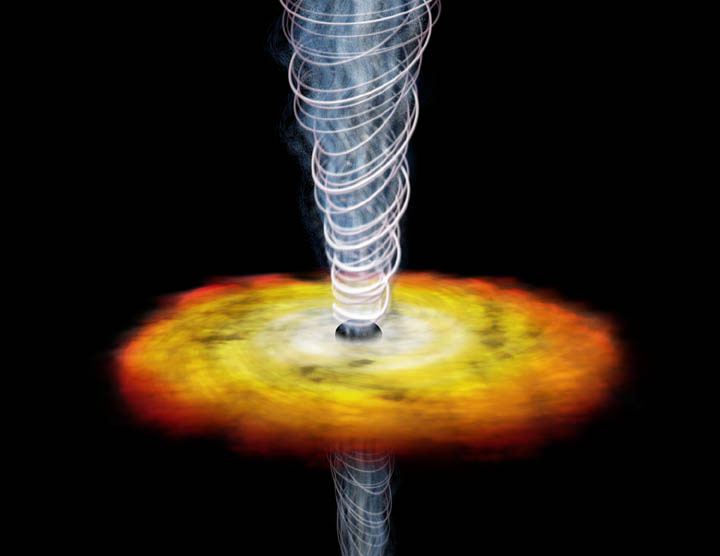
\includegraphics[width=10cm]{Imgs/quasar_illustration}
	\caption{Künstlerische Darstellung eines Quasars\cite{wikiQuasar1}}
	\label{fig:darstQuasar}
\end{figure}
  %!TEX root = bachelor_thesis.tex

\chapter{Entdeckung und Namensgebung}
\label{chapter-kapitel1}

Historisch bezeichnete der Begriff kosmische Radioquellen, die in den 1950er Jahren nicht als Radiogalaxien identifiziert werden konnten, sondern in optischen Beobachtungen blau und „sternförmig“ (also nicht flächig) erschienen. 1963 stellte Maarten Schmidt fest, dass die Radioquelle 3C 273 kein naher Stern ist, sondern mit einer Rotverschiebung von 0,158 im Bereich ferner Galaxien liegt, also nur \textit{quasi} sternartig ist. Spätere Beobachtungen zeigten, dass die hellen sternartigen Quasare doch in die Kerne von Galaxien eingebettet sind, die aber wegen der großen Entfernung schwach erscheinen. Durch die starke Rotverschiebung aufgrund der Expansion des Universums wurden Quasare als sehr weit entfernte Objekte erkannt. Diese Folgerung konnte seit der Entdeckung von Gravitationslinsen unabhängig bestätigt werden. Quasare wurden inzwischen bis zu einer Rotverschiebung von 7,1 entdeckt.

\begin{figure}[h]
	\centering
	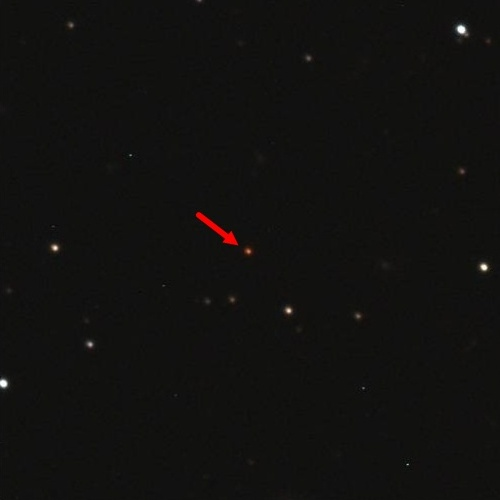
\includegraphics[width=5cm]{Imgs/QSO_APM_08279+5225_marked}
	\caption{Fotografische Aufnahme des Quasars APM08279+5225\\\hspace*{3cm}(Rotverschiebung z=3,9)\cite{wikiQuasar2}}
	\label{fig:darstQuasar}
\end{figure}

Mit der im Jahr 2010 gemachten Entdeckung, dass der 1,6 Mrd. Lichtjahre entfernte Quasar SDSS J0013+1523 als Gravitationslinse für eine 5,9 Mrd. Lichtjahre dahinter liegende Galaxie wirkt, ergibt sich eine direkte Möglichkeit zur Massenbestimmung eines Quasars.[1][2]

Die Bezeichnung \textit{QSO (quasi-stellar object)} schließt nicht nur die klassischen \textit{radiolauten} Quasare ein, sondern auch \textit{radioleise} Objekte mit schwacher Radioemission, aber sonst ähnlichen Eigenschaften. Häufig wird aber der Begriff Quasar etwas ungenau für beide Klassen benutzt.
  %!TEX root = bachelor_thesis.tex

\chapter{Physikalische Eigenschaften}
\label{chapter-kapitel2}

Da Quasare trotz ihrer großen Entfernung relativ hell erscheinen, gehören sie zu den leuchtkräftigsten Objekten im Universum. Nur sehr kurzzeitig hell aufleuchtende Phänomene (Supernova, Gammastrahlenblitz) sind möglicherweise energiereicher. Quasare sind über weite Bereiche der elektromagnetischen Strahlung hell und haben charakteristische Spektren mit sehr breiten Emissionslinien, die in rascher Bewegung befindliches Gas anzeigen.

Quasare gehören wie die schwächeren Seyfertgalaxien zur Klasse der aktiven Galaxien. Die Trennung anhand der Leuchtkraft ist rein historisch bedingt. Nach heutiger Annahme befindet sich im Zentrum aller Galaxien mit einem Bulge ein sehr massereiches Schwarzes Loch, das mehrere Millionen bis Milliarden Sonnenmassen umfassen kann. Aktive Galaxien unterscheiden sich von normalen Galaxien dadurch, dass dieses Schwarze Loch mit der Zeit an Masse zunimmt, da Materie aus der umgebenden Galaxie (interstellares Gas oder zerrissene Sterne) durch die Gravitation des Schwarzen Loches angezogen wird. Dieser Vorgang des Ansammelns von Materie wird in der Astronomie Akkretion genannt. Aufgrund der Drehimpuls­erhaltung bei der einfallenden Materie kann diese nicht direkt in das Schwarze Loch fallen, so dass sich um dieses herum eine Akkretionsscheibe bildet. Durch Reibung heizt sich diese Scheibe auf, wobei gleichzeitig Teile der Materie Drehimpuls verlieren und so in das Schwarze Loch fallen können. Die Emission der aufgeheizten Akkretionsscheibe ist das, was man als typische Strahlung des Quasars beobachtet. Sie kann eine Leuchtkraft ähnlich der von vielen Milliarden Sternen erreichen und somit mehr Licht abstrahlen als die gesamte umgebende Wirtsgalaxie. Die leuchtkräftigsten Quasare erreichen bis über $10^{14}$-fache Sonnenleuchtkraft.

Sofern die Akkretionsscheibe über ein starkes Magnetfeld verfügt, wird ein kleiner Anteil des Materiestromes in zwei Teile gerissen und in Bahnen entlang der Feldlinien des Magnetfeldes gezwungen. Anschließend werden beide Ströme senkrecht zur Ebene der Akkretionsscheibe (einer auf jeder Seite) mit relativistischer Geschwindigkeit in die umgebende Galaxie und den weiteren Weltraum abgestoßen. Diese Jets können im Radiowellen­längenbereich beobachtet werden.
  %!TEX root = bachelor_thesis.tex

\chapter{Zusammenfassung und Ausblick}
\label{chapter-fazit}

Zusammenfassend sind grundlegende Aspekte der Quasare erläutert worden und eine zukünftige Forschung in diesem Bereich weiterhin anzustreben.

  \backmatter

%  \cleardoublepage
%  \phantomsection
%  %\pdfbookmark{Abbildungsverzeichnis}{listoffigures}
%  \listoffigures
%
%  \cleardoublepage
%  \phantomsection
%  %\pdfbookmark{Tabellenverzeichnis}{listoftables}
%  \listoftables
%
%  \cleardoublepage
%  \phantomsection
%  %\pdfbookmark{Definitions- und Theoremverzeichnis}{listoftheorems}
%  \renewcommand{\listtheoremname}{Definitions- und Theoremverzeichnis}
%  \listoftheorems[ignoreall,show={Lemma,Theorem,Korollar,Definition}]

  \cleardoublepage
  \phantomsection

  \nocite{wik16, mil85, mpi16}  
  
  \pdfbookmark{Literaturverzeichnis}{bibliography}
  \bibliography{literature}
\end{document}
